\chapter{Introduction}
(8-Bit) Computers

silicon


Developing an 8-bit Computer Architecture, and its simulation code, just like if I would make a chip. 
While the 8-bit arch should follow the, under my impression the two most important conceptsa
\section{Theory}
\subsection{Turing equivalence}
\cite{turing1936a}

\subsection{The von Neuman Architecture}
\cite{vonneuman1945a}

Following The Von Neumann the architecture shall be structured in a number of modules, the arithmetic logic unit (ALU), the control unit (CU), memory, input and output. The modules interact with each over the three buses, sharing data, address and control signals. All actions are orchestrated by the control unit, signalling the other modules when to read or write data, when to perform calculations, and when to output data, based on the microinstructions stored in the control unit.

\begin{figure}[H]
  \begin{center}
    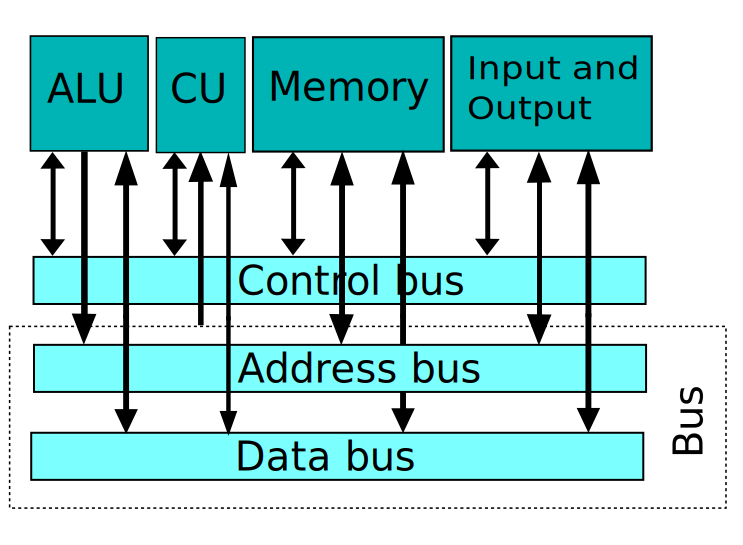
\includegraphics[width=0.5\textwidth]{figures/VNA}
  \end{center}
  \caption{The Von Neumann Architecture. Adapted from \cite{fig-vna}}\label{fig:vna}
\end{figure}

The pioneering approach of the Von-Neumann-Architecture was to store the instructions in the same physical memory, thus accessed in the same way, as the data which simplified the programming process by allowing other programs (compilers, interpreters) to translate from more abstract languages. As instructions and data are stored in the same memory, they must also share the same physical bus. This however leads  to a phenomenon known as the \textit{von Neumann bottleneck} \cite{cit.needed}, where the bus and memory are the limiting factor in the speed of the computer. 

The \textit{von Neumann bottleneck} arises because both the instruction fetch and all data operations must share the same bus and can only occur one after the other, creating a point of congestion. When taking into account that (random access) memory retrieval takes significantly longer than any other operation this bottleneck can be alleviated by introducing a secondary form of memory. Deviating from the Von-Neumann-Architecture the memory module shall be split up into to two modules, a random access memory, storing data and instructions referenced by addresses and the registers, storing a single bus width of data. As well as a number of registers, storing operand data for the alu. The registers function without an address and are directly operated by the control unit.

The modules, in which this architecture is split up to, thus are the ALU, the CU, the memory, the register and the input and output. 

\begin{figure}[H]
  \begin{center}
    \includegraphics[width=0.5\textwidth]{figures/VNA-Adapted}
  \end{center}
  \caption{The Von Neumann Architecture. Adapted from \cite{fig-vna}}\label{fig:vna-adapted}
\end{figure}

The combined address and data bus is from here on out refered to as the bus.

\subsection{Instruction Hierarchy}
- Unless someone programs a compute its a useless piece of crap
- macro instructions
- one macro is however infact multiple micro instructions 
A microinstruction is typically referring to the state of all control signals and is typically generated by the microcode. As it would be extremely inefficient, due to repetition, to only program a computer with individual control signals, the control signals are grouped into microinstructions. The microinstructions are then generated by a net of logic gates or a storage depending on the macro instruction and the current state of the computer.


\subsection{Requirements (or RQB)}
\subsection{Hardware Description Languages}
With the development of highly complex chip designs in the late 20th century further and further abstraction of the process was required, ensuring that all stakeholders knew the exact specifications of the design. \cite{1214355} Whilst the earliest chip designs were drawn by hand and transferred onto silicon by photolithography, chip designs nowadays are written in an abstract computer language; a Hardware Description Language. Apart from allowing separation, modularity and reusability of components, this description later also allowed for simulation of the design and thus a reduction of errors in the final physically built design. 

To ensure that the design correctly implements all features, professional chip designs are fully and automatically tested, by simulating real world conditions as well as corner cases. 
\subsection{Automated Testing}
RBT

\subsection{Development Operations and Version Control Systems}

\section{Idea and Goal}


Motivated by reuniting the the technology that made the personal computing revolution a reality and the earliest theoretical framework of the computer, the goal of this project is to: 
\begin{itemize}
  \item Have a functioning computer architecture that:
 \begin{enumerate}
    \item Has an 8-bit bus width; and
    \item Is Turing complete; and
    \item Is based on the Von-Neumann-Architecture (VNA); and
    \item Implements the Von-Neumann-Cycle; and
    \item Implements features wanted by me; and  
    \item Is kept as simple as possible; and
    \item Is, with supporting work, explainable graphically.
  \end{enumerate}
  \item Have a simulation of this computer architecture that: 
  \begin{enumerate}
    \item Is fully tested, ensuring all requirements are met; and
    \item Is kept as simple as possible; and
    \item Can be interacted with by a user; and
    \item Is programmable by a higher level language (assembly); and
    \item Is, with supporting work, explainable graphically.
  \end{enumerate}
  
\end{itemize}

The limitation on the bus width ensures that the complexity of the architecture is limited and can be grasped by a single person.

\section{Tools}

The most popular flavor of such an \textit{HDL} is Verilog, as defined in \cite{10458102} and its extensions. Given widespread professional use of Verilog, more specifically the Verilog superset SystemVerilog, seemed to be the best option for this project, a large amount of information and guides on the topic exist. The terms SystemVerilog and Verilog will be used interchangeably. 

As \cite{10458102} only defines the language's syntax, a Verilog tool suite is required. Although previous experience in the usage of Verilog exists, expertise on the intricacies of Verilog simulation is still limited. It was thus decided based on the integration with other tooling, as to which suite is to be used. 

The key feature of the chosen suite is the compilation of the Verilog code to a binary and the generation of an interface to C++. Apart from being able to rely on previous experience in C++, it also allows me to make use of a vast ecosystem of testing, code coverage and DevOps frameworks. I chose the GoogleTest framework for my unit testing. 

Additionally, Verilator counts activations of specific lines of code which is used to produce a report that visualizes all used lines of code. This report can help understand if and how tests cover all possible code behaviors. 

\subsection{Verilog Crash Course - Change title}
What differentciates simulated Verilog from other computer languages is its non linear execution and lacks the concept of a main function. Verilog files are not necessarily executed from top to bottom but execution is based on propagation of signals throught the interconnected modules. 

A module is declared with the \texttt{module} keyword. To complete a declaration the module must be named and ports specified. Ports are the connections going in and out of a module. They can either be an \texttt{input}, an \texttt{output} or bidirectional, denoted by \texttt{inout}. Ports are then specified like any other variable, by specifying the datatype, length and name. For this paper usage of datatypes shall be limited to, \texttt{wire}, \texttt{reg} and for readability reasons \texttt{enum}. After the declaration of the ports the body of the module is defined, which contains the module logic.
\begin{lstlisting}
module <module_name> (
  input wire <input_name>,
  output reg <output_name>
);
<module_body>
endmodule
\end{lstlisting}

The following is not intended to be an exhaustive guide to Verilog, but just highlights the most important features and concepts. 

Most digital circuits are based around a clock signal and thus have to exectue operations at every clock cycle. Verilog provides a way to model this with \texttt{always} blocks. Once the condition in the bracket is met, the code block is executed. Apart from simple boolean conditions, the block can also be executed at the rising and falling edge of a signal by using the \texttt{posedge} and \texttt{negedge} keywords.

\begin{lstlisting}
always @(<condition>) begin
  <always_body>
end

\end{lstlisting}

For logic the Verilog standard specifies comparable to other computer or programming languages if-blocks, loops, case statements and various logic and arithmetic operators. Unlike other languages, there are multiple types of assignments in Verilog. The easiest to understand is the continous assignment with the \texttt{assign} keyword. This continously assigns the value of the right hand side to the left hand side comparable to physical wires being connected together through logic gates. If the input changes, the output will change with it nearly instantaneously. The blocking assignment, denoted by the \texttt{=} operator, is used to assign values to variables instantaneously, like in other programming languages. The non-blocking assignment, denoted by the \texttt{<=} operator, only actually assigns the value to the left hand side once the timing step, so every calculation in the current time step, is finished. 

The SystemVerilog standard also specifies a number of additional functions that are not sythesizable, so cannot be translated into hardware, but are useful for simulation, such as \texttt{\$display} and \texttt{\$finish}.

\subsection{Development Environment}
To reproduce the development environment for this project, the following packages need to be installed. I suggest to use Debian 12. 

\begin{itemize}
  \item verilator@5.24
  \item a C++ toolchain (e.g. gcc)
  \item cmake
  \item ninja
\end{itemize}
  

